% This file was created by matplotlib2tikz v0.6.16.
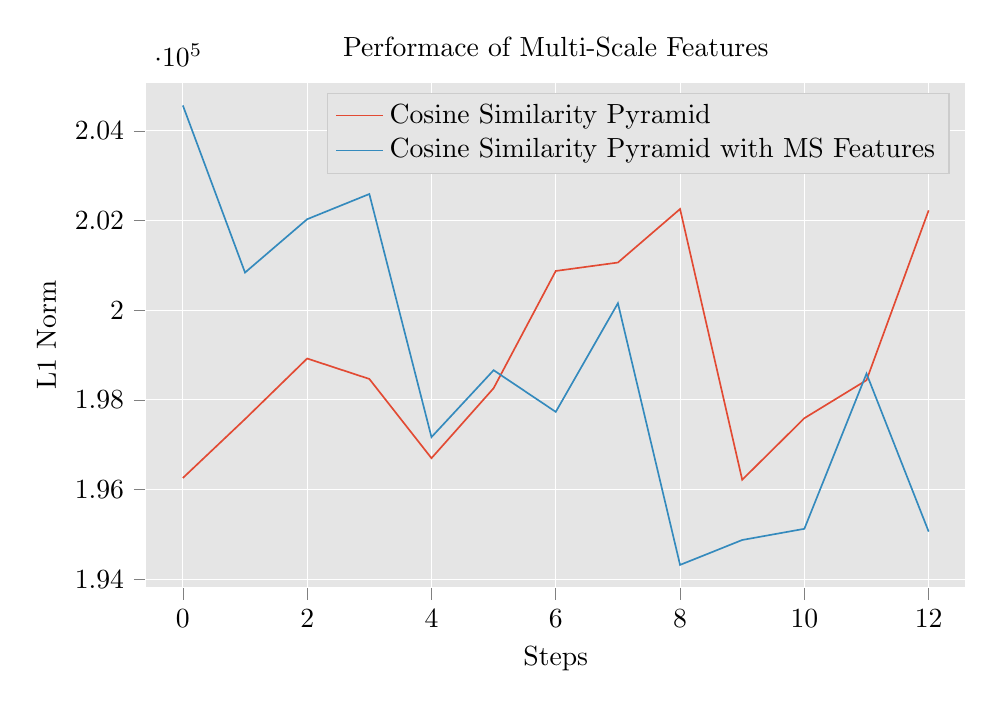
\begin{tikzpicture}

\definecolor{color1}{rgb}{0.203921568627451,0.541176470588235,0.741176470588235}
\definecolor{color0}{rgb}{0.886274509803922,0.290196078431373,0.2}

\begin{axis}[
title={Performace of Multi-Scale Features},
xlabel={Steps},
ylabel={L1 Norm},
xmin=-0.6, xmax=12.6,
ymin=193805.93828125, ymax=205080.57734375,
width=12cm,
height=8cm,
tick align=outside,
tick pos=left,
xmajorgrids,
x grid style={white},
ymajorgrids,
y grid style={white},
axis line style={white},
axis background/.style={fill=white!89.80392156862746!black},
legend style={draw=white!80.0!black, fill=white!89.80392156862746!black},
legend entries={{Cosine Similarity Pyramid},{Cosine Similarity Pyramid with MS Features}},
legend cell align={left}
]
\addlegendimage{no markers, color0}
\addlegendimage{no markers, color1}
\addplot [semithick, color0]
table {%
0 196258.0625
1 197571.0625
2 198923.0625
3 198467.046875
4 196699.53125
5 198260.65625
6 200876.03125
7 201064.0625
8 202257.921875
9 196217.9375
10 197591.296875
11 198439.125
12 202228.28125
};
\addplot [semithick, color1]
table {%
0 204568.09375
1 200840.40625
2 202030.71875
3 202592.6875
4 197169.65625
5 198661.828125
6 197732.484375
7 200156.921875
8 194318.421875
9 194874.515625
10 195123.984375
11 198586.671875
12 195061.6875
};
\end{axis}

\end{tikzpicture}